\section{Design}
This chapter describes the general design of Tsukiji.
Motivations for the choices in our design will be discussed.
For more detailed issues during the process of implementation, see section \ref{implementation}.

\subsection{Architecture}
Tsukiji consists of two main modules (orderbook and trader), a cryptography module, and several smaller utility modules.
This is depicted in figure \ref{modulesfig}.
There are several third-party libraries Tsukiji depends on.
The important ones are described later on in section \ref{dependencies}.

The trader module consists mainly of the Trader class.
Its main purpose is to communicate with other remote Traders.
The Trader class is a subclass of the DatagramProtocol class provided by the Twisted library.
This means the Trader class implements the UDP protocol.
The UDP protocol is the transport protocol used to connect with other traders.
For more information on the application protocol used, see section \ref{protocol}.

The orderbook module has two main functionalities: 1. message creation for the application protocol and 2. managing the state of the orderbook itself and matching bids and asks.
The two are closely related, e.g. matching an ask with a bid produces a trade message.
An example of a function in the first category is the function \texttt{create\_ask(price, quantity, timeout)}.
This function creates an 'ask' message, with a given price, quantity, and timeout.
An example of a function in the second category is the function \texttt{match\_bid(bid)}.
Given a bid as input, check if there are compatible asks from yourself and output the most favourable one.
Other functions are similar in setup.
For more detail, it is best to look at the code itself and its accompanying comments.

The cryptography module contains everything related to actions with public-key cryptography.
At the moment, it mostly functions as a wrapper around the PyCrypto library, for easier use within Tsukiji.
More on this can be read in section \ref{publickeycryptography} and in section \ref{sprint1:identifiers}.

\subsubsection{Dependencies}
\label{dependencies}

% Twisted
% PyCrypto

\subsection{Protocol}
\label{protocol}

\subsection{Public-key cryptography}
\label{publickeycryptography}

\begin{figure}
  \centering
  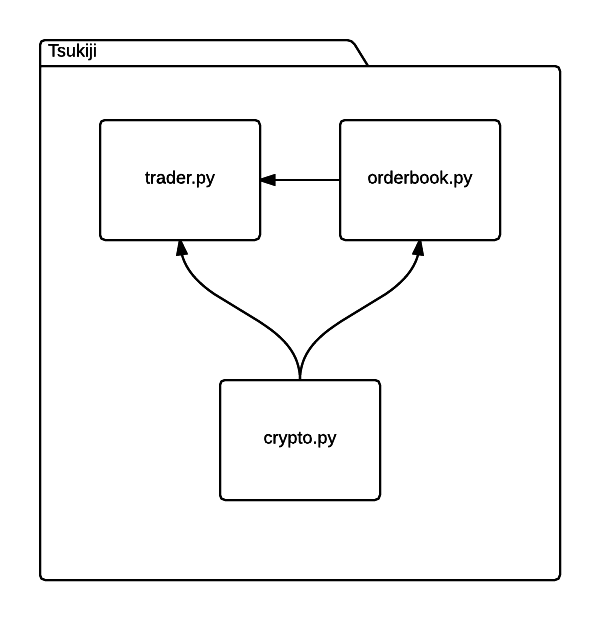
\includegraphics[width=\textwidth]{modules}
  \caption{A diagram with all of Tsukiji's modules}
  \label{modulesfig}
\end{figure}
% Code base
% Protocol
% Cryptography